\documentclass[10pt,a4paper]{article}
\usepackage{inputenc}
\usepackage{graphicx}
\usepackage[french]{babel}
\usepackage[T1]{fontenc}

\usepackage{fontspec}

\usepackage{lmodern}


\usepackage{vmargin}
\usepackage{graphicx}
\usepackage{tabularx}
\setlength{\parindent}{0mm}

\renewcommand{\arraystretch}{2}

%6 pages maximum
\begin{document}

\titlepage{
	\today \vspace{7cm}
	\begin{flushright}\sf\Huge
	{\bfseries LSINF1250} \\[2mm]
	{\bfseries Projet PageRank} \\[1pt]
	{\huge Ranking de réseaux sociaux et page web}
	\end{flushright}
	\ \\[8cm]
	\textbf{Groupe 8} \\
	Denauw Antoine\\
	De Carvalho Borges Antonio
}



\newpage

\section{Procédure Java}
%Explication de la procédure JAVA
\section{Algorithme utilisé}

\paragraph{}La méthode que nous avons choisi est l'algorithme PageRank utilisant la PowerMethod comme présenté au cours (cf. Chapitre 10): METS CE QUE chaque termes signifient avec ce qu'on a noté dans ton bloc non ???
\begin{center}
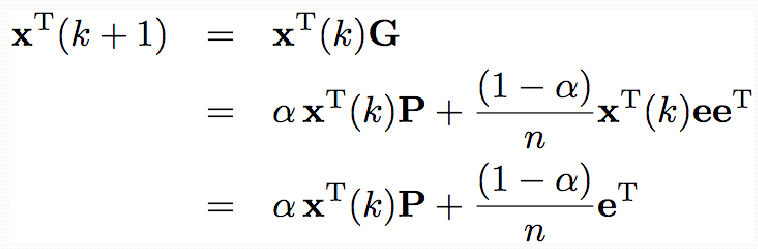
\includegraphics[scale=0.4]{PowerMethod.png} 
\end{center}

%Explication de l'algorithme

\paragraph{}Cette méthode nous a semblé être la plus intuitive et la plus directe pour réaliser cette problématique.

\section{Librairie de calcul matriciel}

\paragraph{}Même que vivement conseillé, nous avons pris la décision de ne pas utiliser de librairie spécifique aux calculs matriciel tel que \textit{JAMA}, mais d'implémenter les différentes fonctions par nous même. Ce choix s'est fait dans une optique de ré-adaptation au langage \textit{JAVA} et de ses règles basiques.

\paragraph{}Pour arriver à reproduire l'algorithme PageRank nous avons dû implémenter les fonctions suivantes:

\hspace{1.5cm}

\begin{itemize}
    \item[•] matrix\_x\_vector : Sers à calculer le vecteur résultant du produit entre une matrice NxN et un vecteur de type Nx1.
    \item[•] degree : Sers à calculer et stocker le degré dans un vecteur de chaque ligne d'une matrice NxN.
    \item[•] multiply (attention à la signature) : Peut servir soit à multiplier un vecteur avec une matrice et un facteur alpha, soit multiplier un vecteur avec un facteur ou bien multiplier deux matrices.
    \item[•] ...
\end{itemize}

\section{Méthode pour déterminer les scores}

%Méthode mathématique ou numérique pour déterminer les scores (avec la formule mathématique)

\paragraph{}La formule mathématique que nous avons décidé d'utiliser est celle de la Power method comme présenté à la section "Algorithme utilisé". Pour cela, nous faisons appel à plusieurs méthode que nous avons implémentées nous même et qui sont aussi expliquée plus haut dans ce document.

\section{Annexe}

\subsection{Scores PageRank}

%Sans téléportation et avec alpha=1 pour les deux graphes tests

\subsection{Code complet}

%Bien le commenter











\end{document}